\lab{Stochastic Differential Equations}{Stochastic Differential Equations}
\label{lab:sde}
\objective{Stochastic differential equations are used to model stochastic processes. 
In this lab we will explore Brownian motion and then derive the Euler-Maruyama numerical method for SDEs.
We will build an Euler-Maruyama numerical solver and use this solver to predict future stock prices.}

Stochastic differential equations combine the concepts of Brownian motion and differential equations in order to model stochastic processes.
A stochastic process is a mathematical object made from a family of random variables.
These processes model events that occur with random changes over time, such as bacterial population growth, movement of gas molecules, and fluctuating stock prices.
To understand stochastic processes, it is imperative to understand Brownian motion.

\section*{Brownian Motion}

Brownian motion is random movement described by the Wiener process.
The Wiener process is a stochastic process $W(t)\sim\mathscr{N}(0,t)$ which satisfies the following conditions:

\begin{enumerate}
\item $W(0)=0$,\\
\item $W(t-s)=W(t) - W(s)$,\\
\item $W(t)$ is independent for all $t$.
\end{enumerate}

For example, imagine a point at zero on a number line.
The point can only move one number away and must move left or right.
The probability of moving left and right is equal and can be modeled by a coin flip.
Let's say that landing on heads moves the point right and tails moves the point left.
On our first flip, we get heads and the point moves from 0 to 1.
Now we flip the coin again.
This coin flip does not depend on the previous coin flip and determines whether the point moves back to 0 or moves to 2.
On the second flip, we get tails and the point moves back to 0.
Continuing this process shows the random movement of the point on the number line.

\begin{figure}
\captionsetup[subfigure]{justification=justified}
\begin{center}
\begin{subfigure}{\textwidth}
\centering
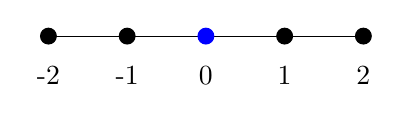
\begin{tikzpicture}
\draw(-2,0)--(-1,0)--(0,0)--(1,0)--(2,0);
\draw[fill] (-2,0) circle [radius=0.1];
\draw[fill] (-1,0) circle [radius=0.1];
\draw[fill, blue] (0,0) circle [radius=0.1];
\draw[fill] (1,0) circle [radius=0.1];
\draw[fill] (2,0) circle [radius=0.1];
\node at (-2,-.5) {-2};
\node at (-1,-.5) {-1};
\node at (0,-.5) {0};
\node at (1,.-.5) {1};
\node at (2,-.5) {2};
\end{tikzpicture}
\caption{Initial position}
\vspace{.3cm}
\end{subfigure}
\begin{subfigure}{\textwidth}
\centering
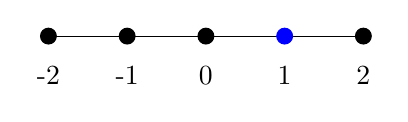
\begin{tikzpicture}
\draw(-2,0)--(-1,0)--(0,0)--(1,0)--(2,0);
\
\draw[fill] (-2,0) circle [radius=0.1];
\draw[fill] (-1,0) circle [radius=0.1];
\draw[fill] (0,0) circle [radius=0.1];
\draw[fill, blue] (1,0) circle [radius=0.1];
\draw[fill] (2,0) circle [radius=0.1];
\node at (-2,-.5) {-2};
\node at (-1,-.5) {-1};
\node at (0,-.5) {0};
\node at (1,.-.5) {1};
\node at (2,-.5) {2};
\end{tikzpicture}
\caption{Heads is flipped and point moves right.}
\vspace{.3cm}
\end{subfigure}
\begin{subfigure}{\textwidth}
\centering
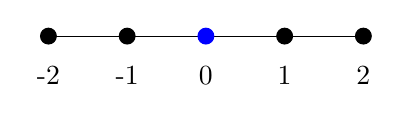
\begin{tikzpicture}
\draw(-2,0)--(-1,0)--(0,0)--(1,0)--(2,0);
\draw[fill] (-2,0) circle [radius=0.1];
\draw[fill] (-1,0) circle [radius=0.1];
\draw[fill, blue] (0,0) circle [radius=0.1];
\draw[fill] (1,0) circle [radius=0.1];
\draw[fill] (2,0) circle [radius=0.1];
\node at (-2,-.5) {-2};
\node at (-1,-.5) {-1};
\node at (0,-.5) {0};
\node at (1,.-.5) {1};
\node at (2,-.5) {2};
\end{tikzpicture}
\caption{Tails is flipped and point moves left.}
\vspace{.3cm}
\end{subfigure}
\begin{subfigure}{\textwidth}
\centering
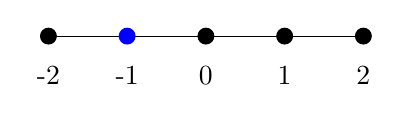
\begin{tikzpicture}
\draw(-2,0)--(-1,0)--(0,0)--(1,0)--(2,0);
\draw[fill] (-2,0) circle [radius=0.1];
\draw[fill, blue] (-1,0) circle [radius=0.1];
\draw[fill] (0,0) circle [radius=0.1];
\draw[fill] (1,0) circle [radius=0.1];
\draw[fill] (2,0) circle [radius=0.1];
\node at (-2,-.5) {-2};
\node at (-1,-.5) {-1};
\node at (0,-.5) {0};
\node at (1,.-.5) {1};
\node at (2,-.5) {2};
\end{tikzpicture}
\caption{Tails is flipped and point moves left.}
\vspace{.3cm}
\end{subfigure}
\caption{Example of Brownian motion. The blue dot travels left or right with equal probability. It is modeled by a coin flip. When heads, the dot moves right. When tails, the dot moves left.}
\end{center}
\end{figure}

As we flip the coin $t$ times, the distribution of the point's position is approximately normally distributed with mean 0 and variance $t$.
Note that $dW\sim\mathscr{N}(0,\Delta t)$ is also approximately normally distributed because $W(t-s)=W(t)-W(s)$ and $W(t-s)\sim\mathscr{N}(0,t-s)$.
Using $dW$, we can show the movement of a point with the differential equation
\begin{equation}
\frac{dS_t}{S_t}=g(t,S_t)dW.
\label{eqn:brownian-motion}
\end{equation}
where $g(t,S_t)$ is a scalar function and $S_t$ is the position of the point at time $t$.
We can manipulate Equation \ref{eqn:brownian-motion} to model the position of the point numerically:


\begin{align*}
dS_t&\approx g(t,S_t)S_tdW\\
S_{t+1}-S_t&\approx g(t,S_t)S_tdW\\
S_{t+1}&\approx S_t+g(t,S_t)S_tdW
\end{align*}
where $dW\sim\mathscr{N}(0,1)$.
This model is itself a stochastic differential equation that is based completely on brownian motion.

\begin{problem}
Write a function \li{brownian_motion()} that accepts a scalar function \li{g}, initial condition \li{y0}, and an array of time points \li{t}.
The function should return an array of the solution to Equation \ref{eqn:brownian-motion} evaluated at $t$.

Animate this function for $g(t,S_t)=1$, $y_0=(1,1)$ and $t\in[0,100)$.
The animation should show a particle moving with a tail indicating it's previous position.

(Hint: Because $y_0\in\mathbb{R}^2$, $dW\in\mathbb{R}^2\times\mathbb{R}^2$ so that each dimension of $y_0$ moves independently. Thus, $dW=\begin{pmatrix}d_{w_1}&0\\0&d_{w_2}\end{pmatrix}$ where $d_{w_i}\sim\mathscr{N}(0,1)$).
\label{prob:brownian-motion}
\end{problem}

\section*{Euler-Maruyama Method}

A stochastic differential equation (SDE) is a differential equation that involves at least one stochastic component.
Equation \ref{eqn:brownian-motion} is an example of a SDE, as its only component is stochastic.
However, most SDEs are not made of just one stochastic component.
A commonly used stochastic differential equation which contains a non-stochastic component is
\begin{equation}
\frac{dS_t}{S_t}=f(t,S_t)dt + g(t,S_t)dW
\label{eqn:general-model}
\end{equation}
where $f(t,S_t)$ and $g(t,S_t)$ are scalar functions and $dW\sim\mathscr{N}(0,\Delta t)$.
In this equation, the first term is a standard differential equation while the second term represents brownian motion.
The combination allows for more accurate models of stochastic processes.
To solve Equation \ref{eqn:general-model}, we apply the Euler-Maruyama method.
This method combines the Euler method for ODEs with an additional stochastic component.
Note that Problem \ref{prob:brownian-motion} is the Euler-Maruyama method where $f(t,S_t)=0$.
We solve for $S_{t+1}$ as follows:

\begin{align*}
dS_t&\approx f(t,S_t)S_tdt + g(t,S_t)S_tdW\\
S_{t+1}-S_t&\approx f(t,S_t)S_tdt + g(t,S_t)S_tdW\\
S_{t+1}&\approx S_t+f(t,S_t)S_tdt + g(t,S_t)S_tdW.
\end{align*}

\begin{problem}
Write a function \li{euler_maruyama()} which accepts a scalar function \li{f}, a scalar function \li{g}, initial condition \li{y0}s, and an array of time points \li{t}.
The function should return an array of the solution to \ref{eqn:general-model}.

To test your function, set $f(t,S_t)=1-(S_t)^2$, $g(t,S_t)=0.1$, $y_0=1$ and $t\in[0,10)$.
Your function should result in a plot which randomly oscillates with $y$ generally in the interval $[0,2]$.
An example is shown in Figure \ref{fig:prob2}.
% try doing histogram instead
\label{prob:euler-maruyama}
\end{problem}

\begin{figure}
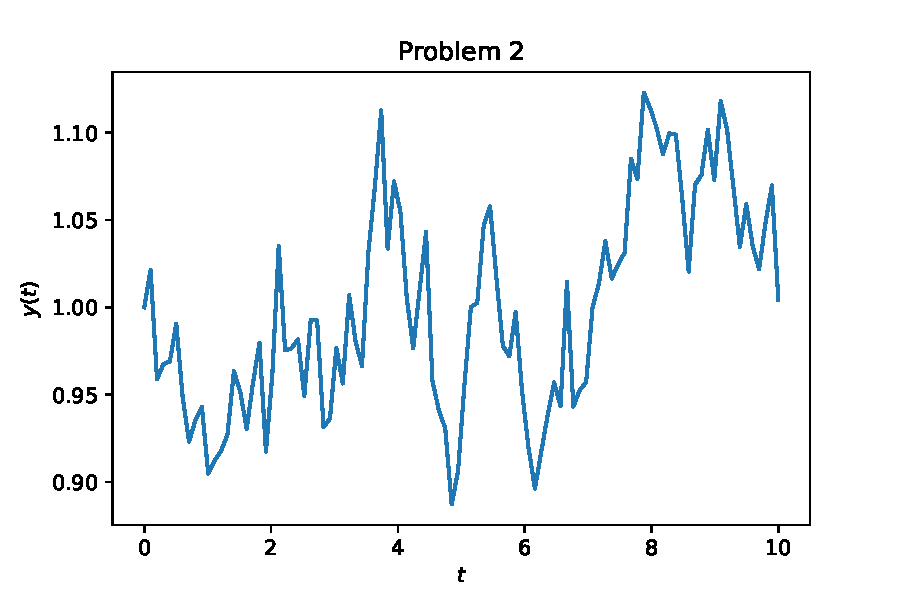
\includegraphics[width=\textwidth]{figures/problem2.pdf}
\caption{Possible solution for $f(t,S_t)=1-(S_t)^2$, $g(t,S_t)=0.1$, $y_0=1$ and $t\in[0,10)$.}
\label{fig:prob2}
\end{figure}

\section*{Drift and Volatility}

SDEs are often used in mathematical finance models.
Particularly, the Geometric Brownian Motion (GBM) model is useful in predicting future stock prices.
The GBM is defined as follows:
\begin{equation}
dS_t=\mu S_tdt+\sigma S_tdW,
\label{eqn:gbm}
\end{equation}
where $\mu$ is the drift of the stock and $\sigma$ is the volatility.
The drift $\mu$ of a stock is the average change in return of historic stock data.
The volatility of a stock is the standard deviation of the change in return of historic stock data.
It is expected that $\mu$ and $\sigma$ will remain the same for future stock data.

To find $\mu$ and $\sigma$, let $\theta=(\mu,\sigma)$.
We want to find $\theta_{MAP}$ (maximum a posteriori) which maximizes the probability that $\mu$ and $\sigma$ fit the historical data.
We can calculate $\theta_{MAP}$ using Bayes Theorem:
\begin{equation}
\theta_{MAP}\Bigg(\frac{dS}{S}\Bigg)=\text{argmax}_\theta P\Bigg(\theta|\frac{dS}{S}\Bigg)=\text{argmax}_\theta\frac{P\Big(\frac{dS}{S}|\theta\Big)P(\theta)}{\int_\Theta P\Big(\frac{dS}{S}|\vartheta\Big)P(\vartheta)d\vartheta}=\text{argmax}_\theta P\Big(\frac{dS}{S}|\theta\Big)P(\theta),
\label{eqn:map}
\end{equation}
where $\Theta$ is the collection of all possible $\theta$.
Since no information is known about $P(\theta)$, we choose $P(\theta)$ to be equal over all $\theta$.
This avoids giving bias to one value of $\theta$ over another.
To ease calculations, we choose our improper prior to be uniformly 1, $P(\theta)=1$.
This implies $\theta_{MAP}=\text{argmax}_\theta P(\frac{dS}{S}|\theta)=\theta_{MLE}$.

Now it is necessary to determine the probability distribution of $P(\frac{dS}{S}|\theta)$.
Plotting the change in stock price results in the following histogram:
\begin{figure}
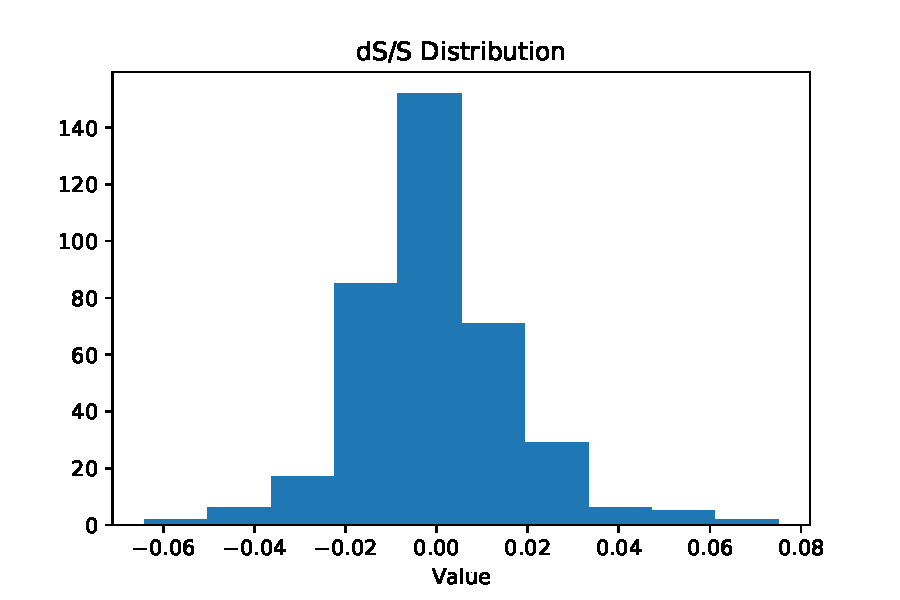
\includegraphics[width=\textwidth]{figures/distribution.pdf}
\caption{Distribution of change in stock price.}
\label{fig:distribution}
\end{figure}
The change in stock price is approximately normally distributed and thus we consider $P(\frac{dS}{S})\sim\mathscr{N}(\mu,\sigma^2)$.
Now we can calculate $\theta_{MAP}$ as follows:

\begin{equation}
\begin{split}
\theta_{MAP}&=\text{argmax}_\theta P(\frac{dS}{S}|\theta)\\
&=\text{argmax}_{\theta}\prod_{i=1}^N\frac{1}{\sqrt{2\pi \sigma^2}}\text{exp}(-\frac{((\frac{dS}{S})_i-\mu)^2}{2\sigma^2})\\
&=\text{argmax}_{\theta}\log(\prod_{i=1}^N\frac{1}{\sqrt{2\pi \sigma^2}}\text{exp}(-\frac{((\frac{dS}{S})_i-\mu)^2}{2\sigma^2}))\\
&=\text{argmax}_{\theta}\sum_{i=1}^N\log(\frac{1}{\sqrt{2\pi \sigma^2}}\text{exp}(-\frac{((\frac{dS}{S})_i-\mu)^2}{2\sigma^2}))\\
&=\text{argmax}_\theta\sum_{i=1}^N\log(\frac{1}{\sqrt{2\pi\sigma^2}})-\frac{((\frac{dS}{S})_i-\mu)^2}{2\sigma^2}\\
&=\text{argmax}_\theta N\log(\frac{1}{\sqrt{2\pi\sigma^2}})-\sum_{i=1}^N\frac{((\frac{dS}{S})_i-\mu)^2}{2\sigma^2}\\
&=\text{argmin}_\theta N\log(\sqrt{2\pi\sigma^2})+\sum_{i=1}^N\frac{((\frac{dS}{S})_i-\mu)^2}{2\sigma^2}\\
&=\text{argmin}_\theta N\log(\sqrt{2\pi\sigma^2})+\frac{1}{2\sigma^2}\sum_{i=1}^N((\frac{dS}{S})_i-\mu)^2
\end{split}
\label{eqn:calculation}
\end{equation}
The end result of Equation \ref{eqn:calculation} gives an equation that can be optimized using \li{scipy.optimize.minimize} to find $\theta$.

\begin{problem}
Write a function \li{theta()} which takes in an array of historical data.
Use \li{scipy.optimize.minimize} and Equation \ref{eqn:calculation} to calculate the optimal $\mu$ and $\sigma$.
Return $\mu$ and $\sigma$.
For the closing stock prices of \li{google_stock.csv}, $\mu\approx1129.4321$ and $\sigma\approx1.8548$.

(Hint: Use the sample mean and sample variance as an initial guess for \li{scipy.optimize.minimize}. Also use \li{method='Nelder-Mead'}.)
\label{prob:theta}
\end{problem}

\begin{problem}
Use \li{euler_maruyama()} to predict the future closing stock prices of Google stock for $t\in[377,427)$.
Plot the original data and the average predicted stock prices.
Return an array of the average future stock prices.
Your plot should look similar to Figure \ref{fig:stock}.

(Hint: Let $f(t,S_t)=\mu$ and $g(t,S_t)=\sigma$. Each $t$ represents one day, so there should be 50 predicted values.)
\label{stock}
\end{problem}

\begin{figure}
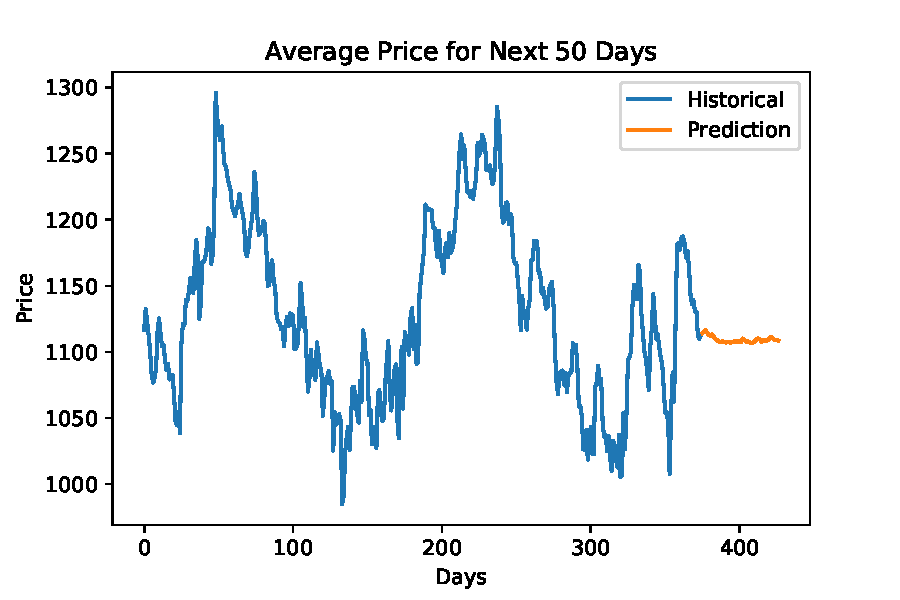
\includegraphics[width=\textwidth]{figures/future_stock.pdf}
\caption{Possible plot of future Google stock prices.}
\label{fig:stock}
\end{figure}

\section*{Convergence of Euler-Maruyama}

The Euler-Maruyama method has strong convergence as $\Delta t\rightarrow\infty$.
This can be seen heuristically by looking at the expected value of the error of the numerical method.
Note equation \ref{eqn:gbm} can be solved analytically to get the solution
\begin{equation}
S(t)=s_0e^{\bigl(\mu-\frac{\sigma^2}{2}\bigr)t+\sigma W(t)}
\label{eqn:analytic}
\end{equation}
where $s_0=S(0)$.
Let $A_{\Delta t}(t)$ be the approximation of $S(t)$ with step size $\Delta t$.
Because we are working with SDEs, we take the expected value of the max error over all $t$ and define the error as

\begin{equation}
E(A_{\Delta t})=\sup_t\mathbb{E}\Bigl(|S(t)-A_{\Delta t}(t)|\Bigr)\approx C(\Delta t)^\gamma.
\end{equation}
where $\gamma$ is the order of convergence and $C$ is some constant.
Taking the log of both sides, we get
\begin{equation}
\log(E(A_{\Delta t}))=\log(C)+\gamma\log(\Delta t).
\end{equation}

To find the order of convergence $\gamma$, we can plot $\Delta t\times E(A_{\Delta t}(t))$ as $\Delta t\rightarrow\infty$ with log axes.
This should result is a straight line with slope $\gamma$, giving us the convergence rate.
For Euler-Maruyama, $\gamma=\frac{1}{2}$.

% Compare to Euler which has convergence of order 1
\begin{problem}
Write a function \li{convergence()} that calculates the convergence of Euler-Maruyama.
Calculate the drift and volatility of the closing prices in \li{google_stock.csv} and use Euler-Maruyama to predict stock values for $t\in[0,50)$.
Calculate the difference between the analytical solution \ref{eqn:analytic} and predicted data from Euler-Maruyama.
Plot the difference for $dt=2^i$ for $i\in[0,1,2,3,4,5]$ on a log-log plot.
Your plot should be a straight line with slope $\frac{1}{2}$.

(Hint: Try using \li{np.arange}).
\end{problem}


